%\subsection{Axiomatics}
\subsection{Soundness \& Completeness}

%In the subsequent discussion, let the Tarski predicate $(\Vdash)$ denote the usual Kripke semantics for the language $\mathcal{L}(\Phi)$ for structures $\langle W, V, P_X, R_{\Box_X}, R_{\BB_X}, R_{\BBI_X}\ra$.  The only unconventional thing we shall doe is to declare $P_X \subseteq W$ and $\mathbb{M},w \vdash \PP_X$ if and only if $w \in P_X$.
%In the subsequent discussion we shall employ the Fraktur typeface (such as $\mathfrak{M}$) to denote models in \textsc{EviL} semantics and the blackboard typeface (such as $\mathbb{M}$) to denote models in Kripke semantics.

From the definitions so far the following can be seen to hold:
\begin{lemma}[Soundness]
If $\vdash \phi$ then for any model $\mathfrak{M}$ and any $(a,A) \in \mathfrak{M}$ we have that $\mathfrak{M},(a,A) \models \phi$ 
\end{lemma}

The proof of the converse, that is \emph{completeness}, proceeds by a three stage construction:
\begin{bul}
\item The first step is to construct a Kripke model $\Cross^\phi$ consisting of finite maximally consistent sets of formulae related to $\phi$ where $\Cross^\phi,w \nVdash \phi$ for some world $w \in W^{\Cross^\phi}$. This model will be shown to make true nine properties.
\item The second step is to construct a model ${\iCross^{\Cross^\phi}}$ which is bisimular to $\Cross^\phi$. This model also makes true these nine properties as well as an additional tenth property.
\item The final third step is to construct an \textsc{EviL} model ${\ipent^{\iCross^{\Cross^\phi}}_\phi}$.
I shall then show that for each $w \in W^{\iCross^{\Cross^\phi}}$ there is a corresponding $(a,A) \in \ipent^{\iCross^{\Cross^\phi}}_\phi$ such that ${\iCross^{\Cross^\phi}}, w \Vdash \psi$ if and only if ${\ipent^{\iCross^{\Cross^\phi}}_\phi},(a,A) \models \psi$ for all subformulae $\psi$ of $\phi$.
\end{bul}
These three steps together suffice to prove completeness.  I shall now proceed to demonstrate these constructions.
\subsubsection{Subformula Model Construction}
In this section we provide definitions and lemmas related to the subformula construction $\Cross^\phi$.  I consciously imitate \citet{boolos_logic_1995} in my approach, as well as the ``Fischer-Ladner Closure'' used in the completeness theorem of PDL \citep{blackburn_modal_2001}.
\begin{mydef}
\begin{eqnarray*}
\sim \phi := \begin{cases} \psi &\textup{ if $\phi = \neg\psi$} \\ \neg \phi & \textup{ o/w} \end{cases} &
\hspace{1cm} \pBB_X \phi := \begin{cases} \phi &\textup{ if $\phi = \BB_X \psi$} \\ \BB_X \phi & \textup{ o/w} \end{cases} \hspace{1cm} &
\pBBI_X \phi := \begin{cases} \phi &\textup{ if $\phi = \BBI_X \psi$} \\ \BBI_X \phi & \textup{ o/w} \end{cases}
\end{eqnarray*}
\end{mydef}
\begin{lemma}\label{equivs2} By Lemma \ref{equivs} we have
\begin{eqnarray*} 
\vdash \sim \phi \IFF \neg \phi &
\hspace{1cm} \vdash \pBB_X \phi \IFF \BB_X \phi \hspace{1cm} &
\vdash \pBBI_X \phi \IFF \BBI_X \phi
\end{eqnarray*}
\ldots moreover \ldots 
\begin{align*}
\pBB_X \phi = \pBB_X\pBB_X \phi & & \pBBI_X\phi = \pBBI_X \pBBI_X \phi \hfill
\end{align*}
\end{lemma}
\begin{mydef} Let $\delta(\phi) \subseteq \mathcal{A}$ be the set of agents that occur in $\phi$\footnote{In natural language, we read $\delta(\phi)$ as ``the dudes mentioned by $\phi$.''} \end{mydef}
\begin{mydef}Define $\Sigma( \Delta,\phi)$ using primitive recursion as follows:
\begin{tabbing}$\Sigma(\Delta,p) :=  \{ p, \neg p, \bot, \neg\bot \} \cup \bigcup\{ \{ \BB_X p, \neg\BB_X p, \BBI_X p, \neg\BBI_X p\} \ |\ X \in \Delta \}$ \\
$\Sigma(\Delta,\bot) := \{ \bot, \neg\bot \}$ \\
$\Sigma(\Delta,\PP_X) := \{ \PP_X, \neg\PP_X, \BB_X \PP_X, \neg \BB_X \PP_X, \bot, \neg\bot \}$ \\
$\Sigma(\Delta,\phi\to\psi) := \{ \phi\to\psi,\neg(\phi\to\psi) \} \cup \Sigma(\Delta,\phi) \cup \Sigma(\Delta,\psi)$ \\
$\Sigma(\Delta,\Nec_X \phi) :=$ \= $\{ \Nec_X \phi, \neg \Nec_X \phi, \BBI_X \Nec_X \phi, \neg\BBI_X\Nec_X \phi \}$ \\
\> $\cup \bigcup\{\{\Nec_X \pBB_Y \phi, \neg\Nec_X \pBB_Y \phi, \Nec_X \pBBI_Y \phi, \neg\Nec_X \pBBI_Y \phi, \pBB_Y \phi, \neg \pBB_Y \phi, \pBBI_Y \phi, \neg\pBBI_Y \phi\}\ |\ Y \in \Delta \}$ \\
\> $ \cup \Sigma(\Delta,\phi)$\\
$\Sigma(\Delta,\BB_X \phi) := \{ \BB_X \phi, \neg\BB_X \phi\} \cup \Sigma(\Delta,\phi)$ \\
$\Sigma(\Delta,\BBI_X \phi) := \{ \BBI_X \phi, \neg\BBI_X \phi\} \cup \Sigma(\Delta,\phi)$
\end{tabbing}
\end{mydef}
\begin{lemma}\label{inclusions}
$\Sigma(\delta(\phi),\phi)$ is finite.  Moreover, we have the following:
\begin{bul}
	\item If $\psi \in \Sigma(\delta(\phi),\phi)$ then $\sim \psi \in \Sigma(\delta(\phi),\phi)$
	\item If $\psi \in \Sigma(\delta(\phi),\phi)$ and $\chi$ is a subformula of $\psi$, then $\chi \in \Sigma(\delta(\phi),\phi)$
	\item If $\BB_X \phi \in \Sigma(\delta(\phi),\phi)$ then $\pBB_X \phi \in \Sigma(\delta(\phi),\phi)$
	\item If $\BBI_X \phi \in \Sigma(\delta(\phi),\phi)$ then $\pBBI_X \phi \in \Sigma(\delta(\phi),\phi)$
\end{bul}
\end{lemma}
\begin{mydef}Let $At(\Psi)$ denote the maximally consistent subsets of $\Psi$
\end{mydef}
\begin{lemma}[Lindenbaum Lemma]If $\Gamma \nvdash \phi$ and $\Gamma\subseteq \Sigma(\delta(\phi),\phi)$, then there is a $\Gamma' \in At(\Sigma(\delta(\phi),\phi))$ such that $\Gamma \subseteq \Gamma'$ and $\Gamma' \nvdash \phi$
\end{lemma}
\begin{mydef}Define $\Cross^\phi := \langle W^{\Cross^\phi}, V^{\Cross^\phi}, P^{\Cross^\phi}_X, R^{\Cross^\phi}_{\Nec_X}, R^{\Cross^\phi}_{\BB_X}, R^{\Cross^\phi}_{\BBI_X}\ra$ where:
\begin{tabbing}
$W^{\Cross^\phi} := At(\Sigma(\delta(\phi),\phi))$ \\
$V^{\Cross^\phi}(p) := \{ w \in W^{\Cross^\phi}\ |\ p \in w \}$ \\
$P^{\Cross^\phi}_X := \{ w \in W^{\Cross^\phi}\ |\ \PP_X \in w \} \cup \{ w\in W^{\Cross^\phi} \ | \ X \nin \delta(A)\}$ \\
$R^{\Cross^\phi}_{\Nec_X} := \{(w,v) \in W^{\Cross^\phi} \times W^{\Cross^\phi}\ |\ \{ \psi\ |\ \Box_X \psi \in w\} \subseteq v \}$\\
$R^{\Cross^\phi}_{\BB_X} := \{(w,v) \in W^{\Cross^\phi} \times W^{\Cross^\phi}\ |$\=$\ \bigcup \{ \{\psi,\pBB_X \psi\}\ |\ \pBB_X \psi \in w\} \subseteq v \wedge \bigcup\{ \{\psi,\pBBI_X \psi\} \ |\ \pBBI_X \psi \in v\} \subseteq w \}$ \\
$R^{\Cross^\phi}_{\BBI_X} := \{(v,w) \in W^{\Cross^\phi} \times W^{\Cross^\phi}\ |$\=$\ \bigcup \{ \{\psi,\pBB_X \psi\}\ |\ \pBB_X \psi \in w\} \subseteq v \wedge \bigcup\{ \{\psi,\pBBI_X \psi\} \ |\ \pBBI_X \psi \in v\} \subseteq w \}$
\end{tabbing}
\end{mydef}
\begin{lemma}[Truth Lemma]\label{truth}
For any subformula $\psi \in \Sigma(\delta(\phi),\phi)$ and any $w \in W^{\Cross^\phi}$, we have that $\Cross^\phi, w \Vdash \psi$ if and only if $\psi \in w$
\end{lemma}
\begin{proof} The proof proceeds by induction on $\psi$.  Most of the steps are routine, with the exception of the right to left directions for the boxes.

I shall demonstrate the right to left direction for $\BB_X$.  Assume that $\BB_X \psi \nin w$, then $w \nvdash \BB_X \psi$.  By Lemma \ref{equivs2} this is true if and only if $w \nvdash \pBB_X \psi$.  Now abbreviate:
\begin{align*}
A := & \bigcup \{ \{\chi,\pBB_X \chi\}\ |\ \pBB_X \chi \in w \}\\
B := & \{ \sim \pBBI_X \chi \ | \ \pBBI_X \chi \in \Sigma(\delta(\phi),\phi) \wedge \sim\chi \in w \}
\end{align*}
Now suppose towards a contradiction that $\{\sim \psi\} \cup A \cup B \vdash \bot$.  Then $A \cup B \vdash \psi$, and furthermore by Lemma \ref{equivs2} and rule (III) from the axioms we have that $\pBB_X A \cup \pBB_X B \vdash \pBB_X \psi$.\footnote{Here $\pBB_X S$ is shorthand for $\{ \pBB_X \chi \ |\ \chi \in S\}$.} But then let 
\begin{align*}
A' := & \{ \pBB_X \chi\ |\ \pBB_X \chi \in w \}\\
B' := & \{ \sim \chi \ | \  \sim\chi \in w \}
\end{align*}
Since $\pBB_X \pBB_X \chi = \pBB_X \chi$ by Lemma \ref{equivs2}, we have $A' = \pBB_X A$.  Moreover, by Lemma \ref{equivs2}, axiom 13, and classical logic we can see that
\[ \vdash \sim \chi \to \pBB_X \sim \pBBI_X \psi \]
Thus for every $\beta \in \pBB_X B$ we have that $B' \vdash \beta$.  Hence by $n$ applications of the Cut rule we can arrive at 
\[ A' \cup B' \vdash \pBB_X \chi \]
However, evidently $A' \cup B' \subseteq w$, hence $w \vdash \pBB_X \psi$, which contradicts what has been stipulated. $\lightning$

Hence it must be that $\{\sim \psi\} \cup A \cup B \nvdash \bot$.  In addition, from the fact that $w \subseteq \Sigma(\delta(\phi),\phi)$ with Lemma  \ref{inclusions} and the hypothesis we have that $\{\sim \psi\} \cup A \cup B \subseteq \Sigma(\delta(\phi),\phi)$.  Hence by the Lindenbaum Lemma we have that there is some $v \in At(\Sigma(\delta(\phi),\phi))$ such that $\{\sim \psi\} \cup A \cup B \subseteq v$.  By the inductive hypothesis we have that $\Cross^\phi, v \nVdash \psi$.

To complete the argument, we have to show that $w R^{\Cross^\phi}_{\BB_X} v$.  Since $A \subseteq v$ we just need to check that $\bigcup\{ \{\psi,\pBBI_X \psi\} \ |\ \pBBI_X \psi \in v\} \subseteq w$.  Suppose that $\pBBI_X \psi \in v$ but $\psi \nin w$.  Since $w$ is maximally consistent we have then that $\nin \psi \in w$.  Thus $\sim \pBBI_X \psi \in v$, which contradicts that $v$ is consistent. $\lightning$  Now suppose that $\pBBI_X \psi \in v$ but $\pBBI_X \psi \nin w$, hence $\sim \pBBI_X \psi \in w$ and thus $\sim \pBBI_X \pBBI_X \psi \in v$.  However we know from Lemma \ref{equivs2} that $\pBBI_X \pBBI_X \psi = \pBBI_X \psi$, which once again implies that $v$ is inconsistent. $\lightning$
\end{proof}

\begin{lemma}[$\Cross^\phi$ is Partly \textsc{EviL}]\label{partly}
$\Cross^\phi$ makes true the following properties:
\begin{mynum}
\item $R^{\Cross^\phi}_{\BB_X} \subseteq W^{\Cross^\phi} \times W^{\Cross^\phi}$
\item $W^{\Cross^\phi}$ is finite
\item For all $w \in W^{\Cross^\phi}$ we have $w R^{\Cross^\phi}_{\BB_X} w$ 
\item If $w R^{\Cross^\phi}_{\BB_X} v$ and $v R^{\Cross^\phi}_{\BB_X} z$ then $v R^{\Cross^\phi}_{\BB_X} z$
\item $R^{\Cross^\phi}_{\BBI_X} = (R^{\Cross^\phi}_{\BB_X})^{-1}$
\item If $w R^{\Cross^\phi}_{\BB_X} v$ then $w \in V^{\Cross^\phi}(p)$ if and only if $v \in V^{\Cross^\phi}(p)$
\item If $w R^{\Cross^\phi}_{\BB_X} v$ and $v R^{\Cross^\phi}_{\Nec_X} u$ then $v R^{\Cross^\phi}_{\Nec_X} u$
\item If $w R^{\Cross^\phi}_{\BB_X} v$ then $u R^{\Cross^\phi}_{\Nec_X} w$ if and only if $u R^{\Cross^\phi}_{\Nec_X} v$
\item If $w\in P^{\Cross^\phi}_X$ then $w R^{\Cross^\phi}_{\Nec_X} w$
\end{mynum}
\ldots for all $\{X,Y\} \subseteq \mathcal{A}$.  Any model with the same modal similarity type as $\Cross^\phi$ that makes the above true is said to be \textbf{partly \textsc{EviL}}

\end{lemma}

Unfortunately, while $\Cross^\phi$ is nearly what is necessary to derive completeness for my semantics, it is not perfect.  Another stage of the construction is necessary.

\subsubsection{Bisimulation}

I first introduce a Backus-Naur form grammar for the $\mathsf{Either}$ type constructor, which may be viewed as a coproduct in category theory (in the category of Sets)\footnote{$\mathsf{Either}$ is taken from the functional programming language \texttt{Haskell}}:
\[ \mathsf{Either}\ a\ b ::= a_l \ |\ b_r \]
%We shall now use this to make a definition.
\begin{mydef}
Let $\mathbb{M}$ be a Kripke model, then define $\invis^\mathbb{M}$ as a model
\[\la W^{\invis^\mathbb{M}},V^{\invis^\mathbb{M}}, P^{\invis^\mathbb{M}}_X,R^{\invis^\mathbb{M}}_{\Nec_X},R^{\invis^\mathbb{M}}_{\BB_X},R^{\invis^\mathbb{M}}_{\BBI_X}\ra\] 
\ldots where \ldots
\begin{tabbing}
$W^{\invis^\mathbb{M}} := \bigcup\{\{w_l,w_r\}\ |\ w\in W^\mathbb{M}\}$\\
$V^{\invis^\mathbb{M}}(p) := \bigcup\{\{w_l,w_r\}\ |\ w\in V^\mathbb{M}(p)\}$\\
$P^{\invis^\mathbb{M}}_X := \bigcup\{\{w_l,w_r\}\ |\  w\in P^\mathbb{M}_X\}$\\
$R^{\invis^\mathbb{M}}_{\Nec_X} := \bigcup\{\{(w_l,v_r),(w_r,v_l)\}\ |\ w R^\mathbb{M}_{\Nec_X} v \wedge w \nin P^\mathbb{M}_X\} \cup \bigcup\{\{w_l,w_r\}\times \{v_l,v_r\}\ |\ w R^\mathbb{M}_{\Nec_X} v \wedge w \in P^\mathbb{M}_X\}$\\
$R^{\invis^\mathbb{M}}_{\BB_X} := \bigcup\{\{(w_l,v_l),(w_r,v_r)\}\ | \ w R^\mathbb{M}_{\BB_X} v \}$ \\
$R^{\invis^\mathbb{M}}_{\BBI_X} := \bigcup\{\{(w_l,v_l),(w_r,v_r)\}\ | \ w R^\mathbb{M}_{\BBI_X} v \}$
\end{tabbing}

\end{mydef}
\begin{lemma}\label{bisimulation}
For any Kripke model $\mathbb{M} = \la W,V,P_X,R_{\Nec_X},R_{\BB_X}, R_{\BBI_X}\ra$, we have the following bisimulation $Z$ between $\mathbb{M}$ and $\invis^\mathbb{M}$:
\begin{eqnarray*} w Z w_l & \& & w Z w_r \end{eqnarray*}
\end{lemma}

\begin{lemma}
If $\mathbb{M}$ is partly \textsc{EviL} then $\invis^\mathbb{M}$ is partly \textsc{EviL} as well.  It also makes true another, novel property: 
\begin{mynum}[start=10,resume]
\item If $w R^{\invis^\mathbb{M}}_{\Nec_X} w$ then $w\in P^{\invis^\mathbb{M}}_X$
\end{mynum}
Any partly \textsc{EviL} Kripke model that makes true this tenth property is said to be \textbf{completely \textsc{EviL}}


\end{lemma}

%\begin{mydef}
%By abuse of notation, we shall abbreviate $\invis^{\Cross^\phi}$ as $\iCross^\phi$
%
%\end{mydef}
\subsubsection{Translation}

In the subsequent discussion, it will be useful to exploit certain properties of \emph{partly \textsc{EviL}} models.  To this end we introduce the concept of a \emph{column}.

\begin{mydef}Let $\mathbb{M}$ be a partly \textsc{EviL} Kripke structure.  I shall make the following definition:
\[ \lcorners w\rcorners^\mathbb{M} := \{ v\ |\ w (R^{\mathbb{M}}_{\BB_X}\cup R^{\mathbb{M}}_{\BBI_X})^\ast v \}\]
\ldots where $R^\ast$ is the reflexive transitive closure of $R$
\end{mydef}

\begin{lemma}[Column Lemma]\label{column}
The following hold if $\mathbb{M}$ is partly \textsc{EviL}:
\begin{mynum}
	\item For all $w$ we have $w \in \lcorners w\rcorners^\mathbb{M}$
	\item If $w \in \lcorners v\rcorners^\mathbb{M}$ then $\lcorners w\rcorners^\mathbb{M} = \lcorners v\rcorners^\mathbb{M}$
	\item If $w R^\mathbb{M}_{\Nec_X} v$ then for all $u \in \lcorners v\rcorners^\mathbb{M}$ we have $w R^\mathbb{M}_{\Nec_X} u$
	\item If $w \in \lcorners v\rcorners^\mathbb{M}$ then $w\in V^\mathbb{M}(p)$ if and only if $v \in V^\mathbb{M}(p)$ for all $p \in \Phi$
\end{mynum}

\end{lemma}

\begin{mydef}
 Let $L(\phi) := \{ p \in \Phi \ |\ p \textup{ is a subformula of } \phi\}$
\\ Let $\ang^\mathbb{M} := \bigcup \{\{\{w\}, \lcorners w\rcorners^\mathbb{M}\} \ |\ w \in W^\mathbb{M}\}$
\\ Let $\rho_\phi^\mathbb{M}: \ang^\mathbb{M} \rightarrowtail \Phi \; \bs\; L(\phi)$ be an injection
\\ Let $\Kill_\phi^\mathbb{M} : W^\mathbb{M} \to \powerset \Phi \times \powerset(\mathcal{L}|_\textsf{Prop}(\Phi))$ be defined such that:
\begin{center}
\begin{minipage}{3in}
\begin{tabbing}
$\Kill_\phi^\mathbb{M}(w) := (\{p \in L(\phi) \ |\ \mathbb{M},w\Vdash p\} \cup \{\rho^\mathbb{M}_\phi(\lcorners w\rcorners^\mathbb{M})\},\lambda X.$\= $\{\neg \rho^\mathbb{M}_\phi(\lcorners v\rcorners^\mathbb{M}) \ |\ \neg w R^\mathbb{M}_{\Nec_X} v\}$\\
\> $\cup \{\bot \to \rho^\mathbb{M}_\phi(\{v\}) \ |\ w R^\mathbb{M}_{\BB_X} v\})$
\end{tabbing}
\end{minipage}
\end{center}
Let $\ipent^\mathbb{M}_\phi := \Kill_\phi^\mathbb{M}[W^\mathbb{M}]$

\end{mydef}

\begin{lemma}\label{translation}
Let $\mathbb{M}$ be a completely \textsc{EviL} Kripke structure.  Then for any subformula $\psi$ of $\phi$ and any $w \in W^\mathbb{M}$, we have $\mathbb{M},w \Vdash \psi$ if and only if $\ipent^\mathbb{M}_\phi, \Kill_\phi^\mathbb{M}(w) \models \psi$

\end{lemma}
\begin{proof}
Apply induction.  The only challenging cases involve the boxes, so we shall illustrate $\Box_X \psi$.  

Assume that $\mathbb{M}, w \nVdash \Box_X \psi$, then there's some $v \in W^\mathbb{M}$ such that $w R^\mathbb{M}_{\Box_X} v$ $\mathbb{M}, v \nVdash \psi$. Let $(a,A) := \Kill^\mathbb{M}(w)$ and $(b,B) := \Kill^\mathbb{M}(v)_\phi$. By the inductive hypothesis it suffices to show that $\ipent^\mathbb{M}_\phi,(b,B) \models A_X$.  But the only things in  $A_X$ are tautologies or formulae of the form $\neg \rho^\mathbb{M}_\phi(\lcorners u\rcorners^\mathbb{M})$ where $\neg w R^\mathbb{M}_{\Nec_X} u$.  But then Lemma \ref{column} it can't be that $\neg \rho^\mathbb{M}_\phi(\lcorners v\rcorners^\mathbb{M}) \in A_X$, and this suffices.

Now assume that $\ipent^\mathbb{M}_\phi, (a,A) \nmodels \Box_X \psi$ where $(a,A) = \Kill^\mathbb{M}(w)$, so there must be some $v \in W^\mathbb{M}$ such that $\ipent^\mathbb{M}_\phi, (b,B) \nmodels  \psi$ where $(b,B) = \Kill^\mathbb{M}(v)$ and $\ipent^\mathbb{M}_\phi, (b,B) \models  A_X$.  By the inductive hypothesis it suffices to show that $w R^\mathbb{M}_{\Nec_X} v$, but this must be the case for otherwise $\neg \rho^\mathbb{M}_\phi(\lcorners v\rcorners^\mathbb{M}) \in A_X$ and then it couldn't be that $\ipent^\mathbb{M}_\phi, (b,B) \models  A_X$ since $\rho^\mathbb{M}_\phi(\lcorners v\rcorners^\mathbb{M}) \in B$.

The inductive steps for the other boxes follow by similar reasoning.
\end{proof}

\subsubsection{Completeness}\label{conservative-extension}

\begin{theorem}
If $\nvdash \phi$ then there is some model $\mathfrak{M}$ and some $(a,A) \in \mathfrak{M}$ such that $\mathfrak{M},(a,A) \nmodels \phi$ 
\end{theorem}
\begin{proof}
	Assume $\nvdash \phi$, then by Lemmas \ref{truth} and \ref{partly} we have some partly \textsc{EviL} Kripke 
	structure and world such that $\mathbb{A},a \nVdash \phi$.  By Lemma \ref{bisimulation} we have that there is a 
	completely \textsc{EviL} Kripke structure $\mathbb{B}$ such that $\mathbb{A}\ \underline{\IFF}{}\ \mathbb{B}$, thus there is some world $b$ such that $\mathbb{B},b \nVdash \phi$.  
	Finally by Lemma \ref{translation} we have that there's a model $\mathfrak{C}$ in \textsc{EviL} semantics and a pair $(c,C) \in \mathfrak{C}$ such that $\mathfrak{C},(c,C) \nmodels \phi$.
\end{proof}

\subsection{Conservativity, Decidability \& Complexity}

In this section, we discuss basic computability results for \textsc{EviL}. I demonstrate that all of the fragments of \textsc{EviL} are decidable, and establish a lower bound on the computational complexity.

I shall first prove the following lemma:

\begin{lemma}
\textsc{EviL}, \textsc{EviL}$^\BM$ and \textsc{EviL}$^\BP$ with a single agent are all conservative extensions of the basic modal logic with just axiom $K$.  That is, if $\nvdash_K \phi$ then $\nvdash_{\textup{\textsc{EviL}}} \phi$ and similarly for the fragments \textsc{EviL}$^\BM$ and \textsc{EviL}$^\BP$.

\textsc{EviL} with $m > n$ agents is a conservative extension of \textsc{EviL} with $n$ agents, and likewise for the fragments \textsc{EviL}$^\BM$ and \textsc{EviL}$^\BP$ 
\end{lemma}
\begin{proof}
Assume that $\nvdash_K \phi$, then we know from modal logic that there's a finite Kripke Structure $\mathbb{M} := \langle W, V, R\rangle$ such and a world $w \in W$ such that $\mathbb{M},w \nvdash \phi$.  Now extend $\mathbb{M}$ to $\mathbb{M}' := \langle W, V, P, R_\Nec, R_\BB, R_\BBI \rangle$ where
\begin{bul}
	\item $P := \{(v,v)\ |\ v R v\}$
	\item $R_\BB := R_\BBI := \{(w,w)\ |\ w \in W\}$
\end{bul}
\ldots this model is trivially completely \textsc{EviL}. Moreover we know that $\mathbb{M}$ is an elementary submodel of $\mathbb{M}'$, so $\mathbb{M}', w\nvdash \phi$.  Hence by the Lemma \ref{translation} we have a model $\mathfrak{M}$ and $(a,A) \in \mathfrak{M}$ such that $\mathfrak{M},(a,A) \nmodels \phi$; so by soundness for \textsc{EviL} we have the desired result.

Similarly, if we $\nvdash_{\textup{\textsc{EviL}}_\mathcal{A}} \phi$ then by completeness can find a witnessing $\mathfrak{M}$ and $(a,A) \in \mathfrak{M}$ such that $\mathfrak{M},(a,A) \nmodels \phi$.  But then we can embed $\mathfrak{M}$ into $\mathfrak{M}'$ for agents $\mathcal{B} \supseteq \mathcal{A}$ where $\mathfrak{M}' := \{(a,A') \ |\ (a,A) \in \mathfrak{M}\}$ and
$$ A'_X := \begin{cases} A_X & X \in\mathcal{A} \\ \varnothing & X \nin \mathcal{A}\end{cases} $$
\end{proof}

By similar arguments, \textsc{EviL} is a conservative extension of \textsc{EviL}$^\BM$ and \textsc{EviL}$^\BP$, and that all three of these are conservative extensions of $K$.  This is summerized in the Fig. \ref{conservative-extensions}.

\begin{figure}[ht]
\begin{center}
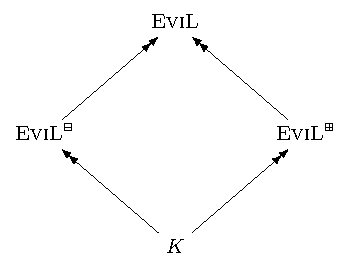
\includegraphics[]{logics/evils.pdf}
\end{center}
\caption{\textsc{EviL} conservative extensions of $K$}
\label{conservative-extensions}
\end{figure}

\begin{lemma}
	\textsc{EviL} is \textsf{PSPACE} hard 
\end{lemma}
\begin{proof}
This follows trivially from the fact that \textsc{EviL} is a conservative extension of basic modal logic, and the decision problem for basic modal logic is \textsf{PSPACE} complete.
\end{proof}